\section{The SEA Technique}
\label{SEC:approach}

\begin{figure}[t]
  \center{}
  \fbox{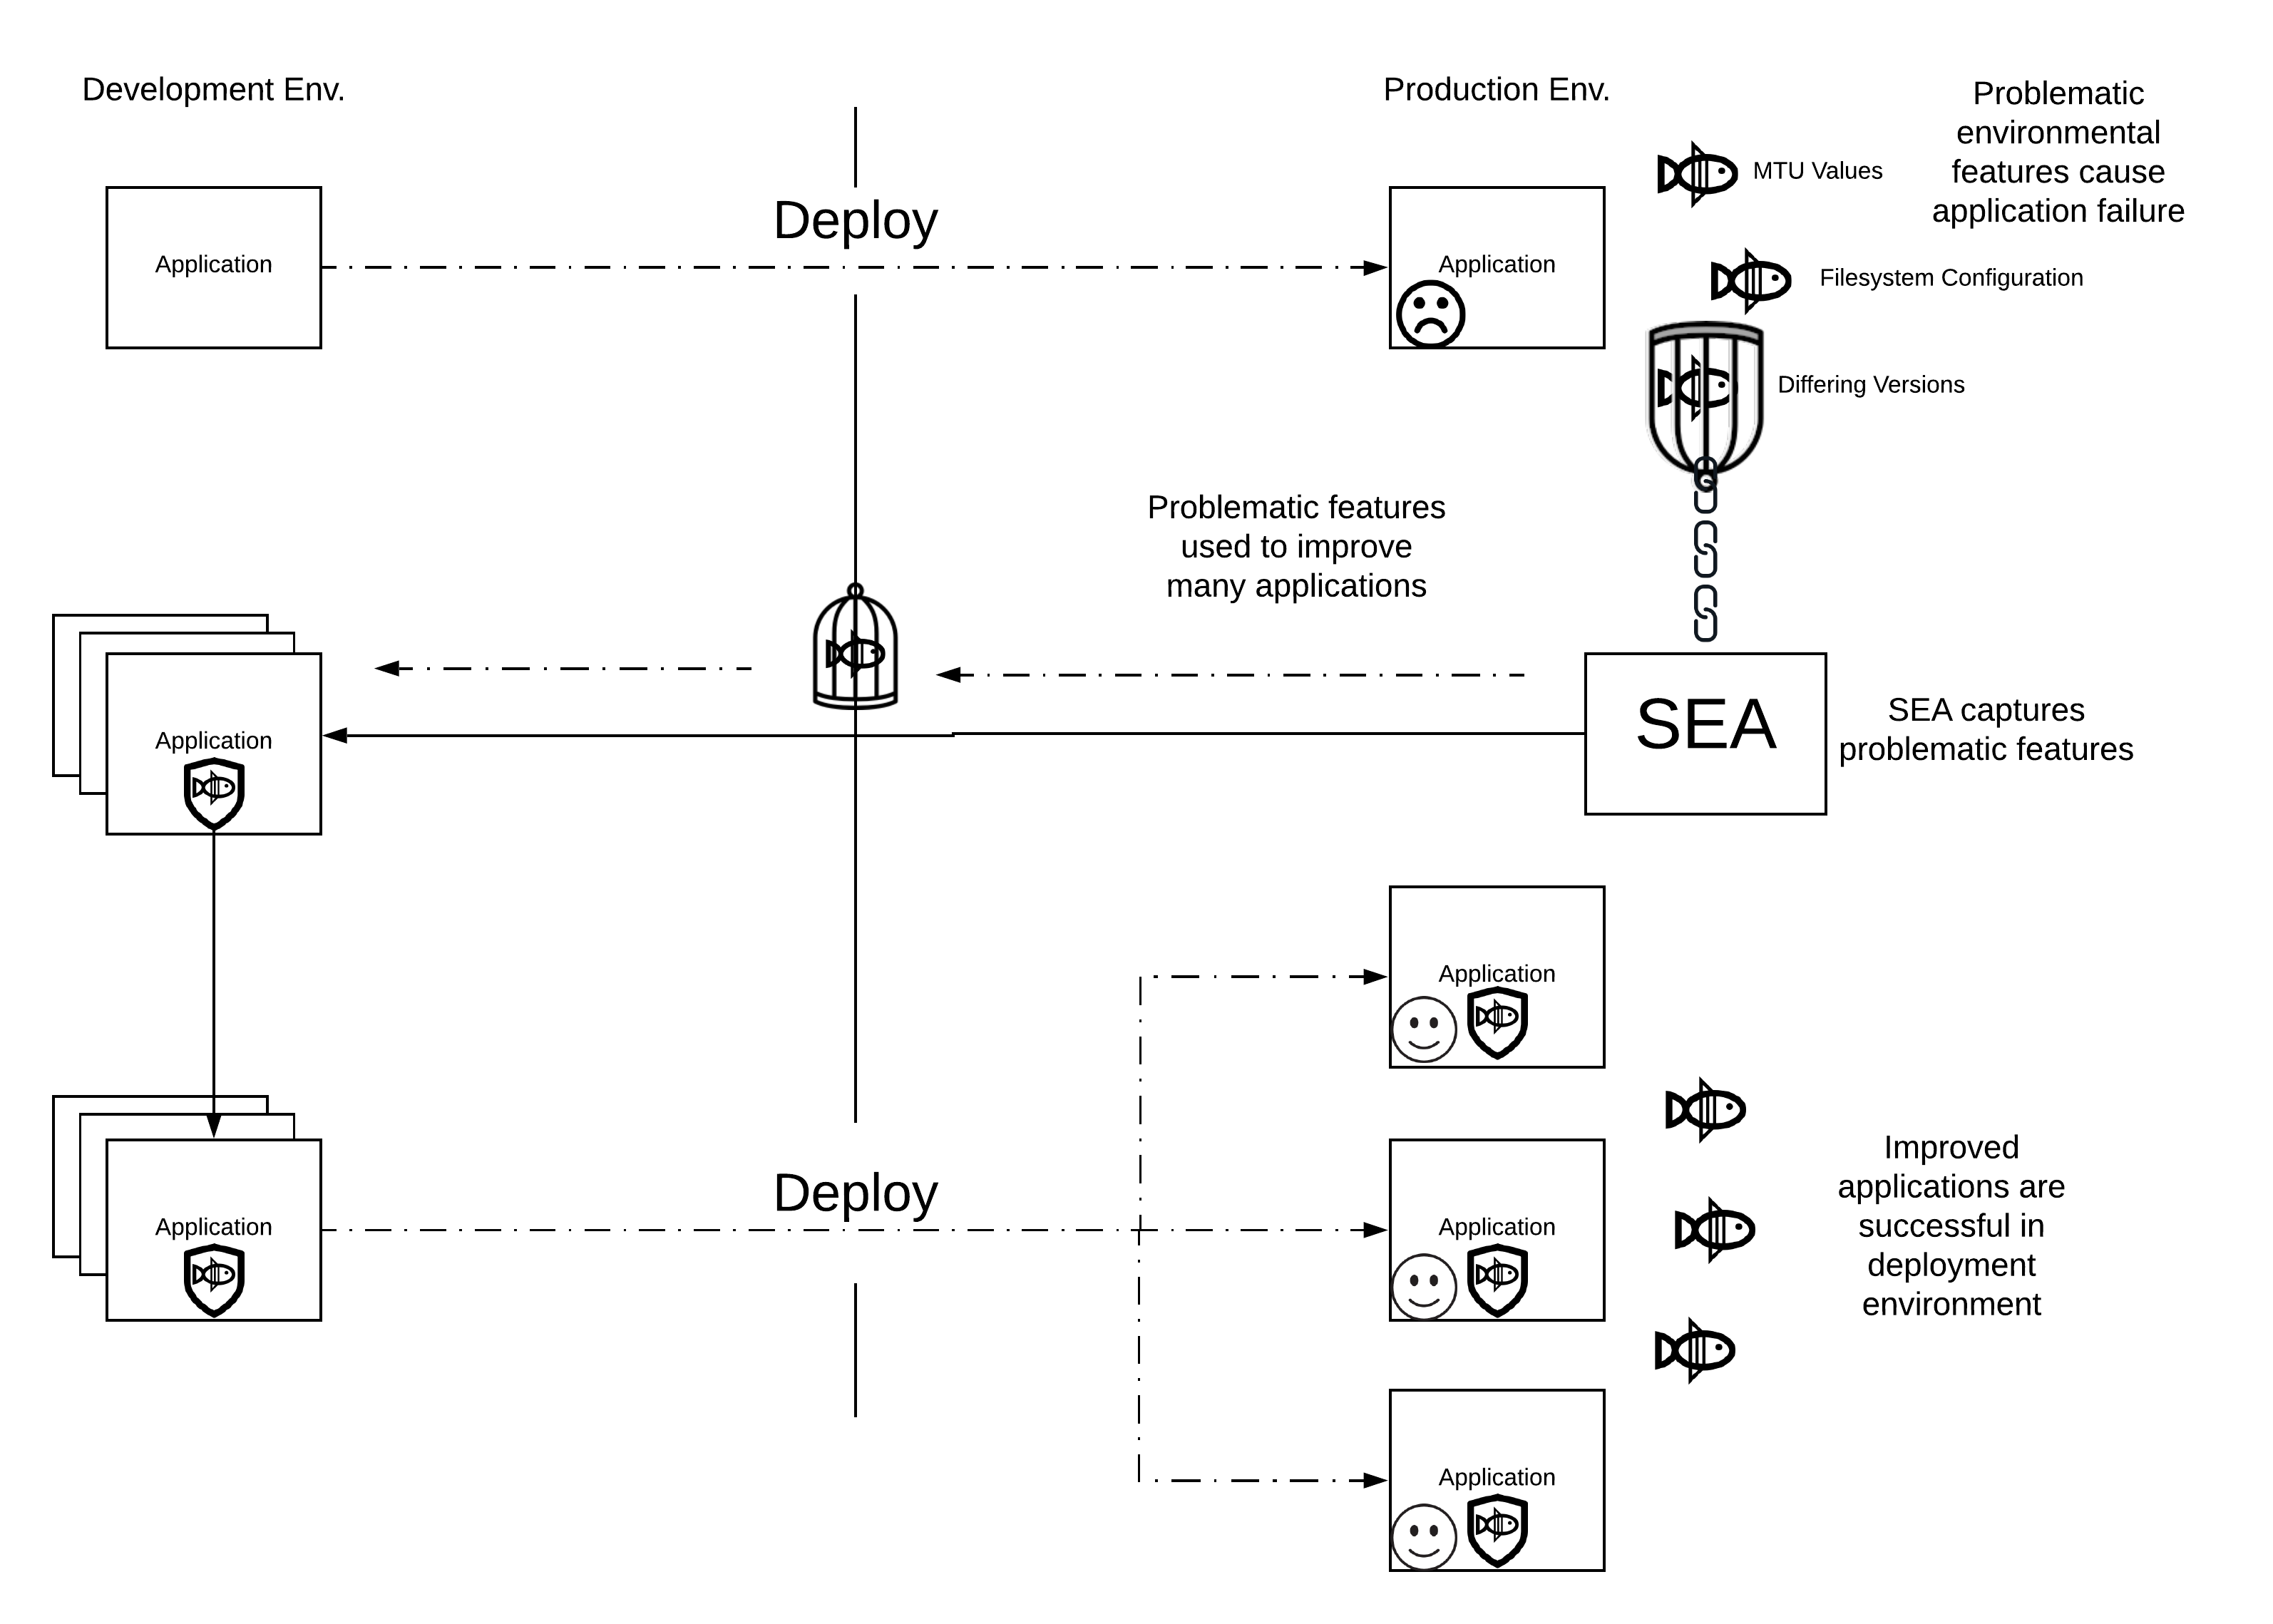
\includegraphics[scale=.37]{images/approach}}
  \caption{Using SEA allows developers to capture features that make an
    environment problematic and use them to prevent future applications
    from falling victim to the bugs of the past.}
  \label{figure:approach}
\end{figure}

\begin{figure*}[t]
  \center{}
  \fbox{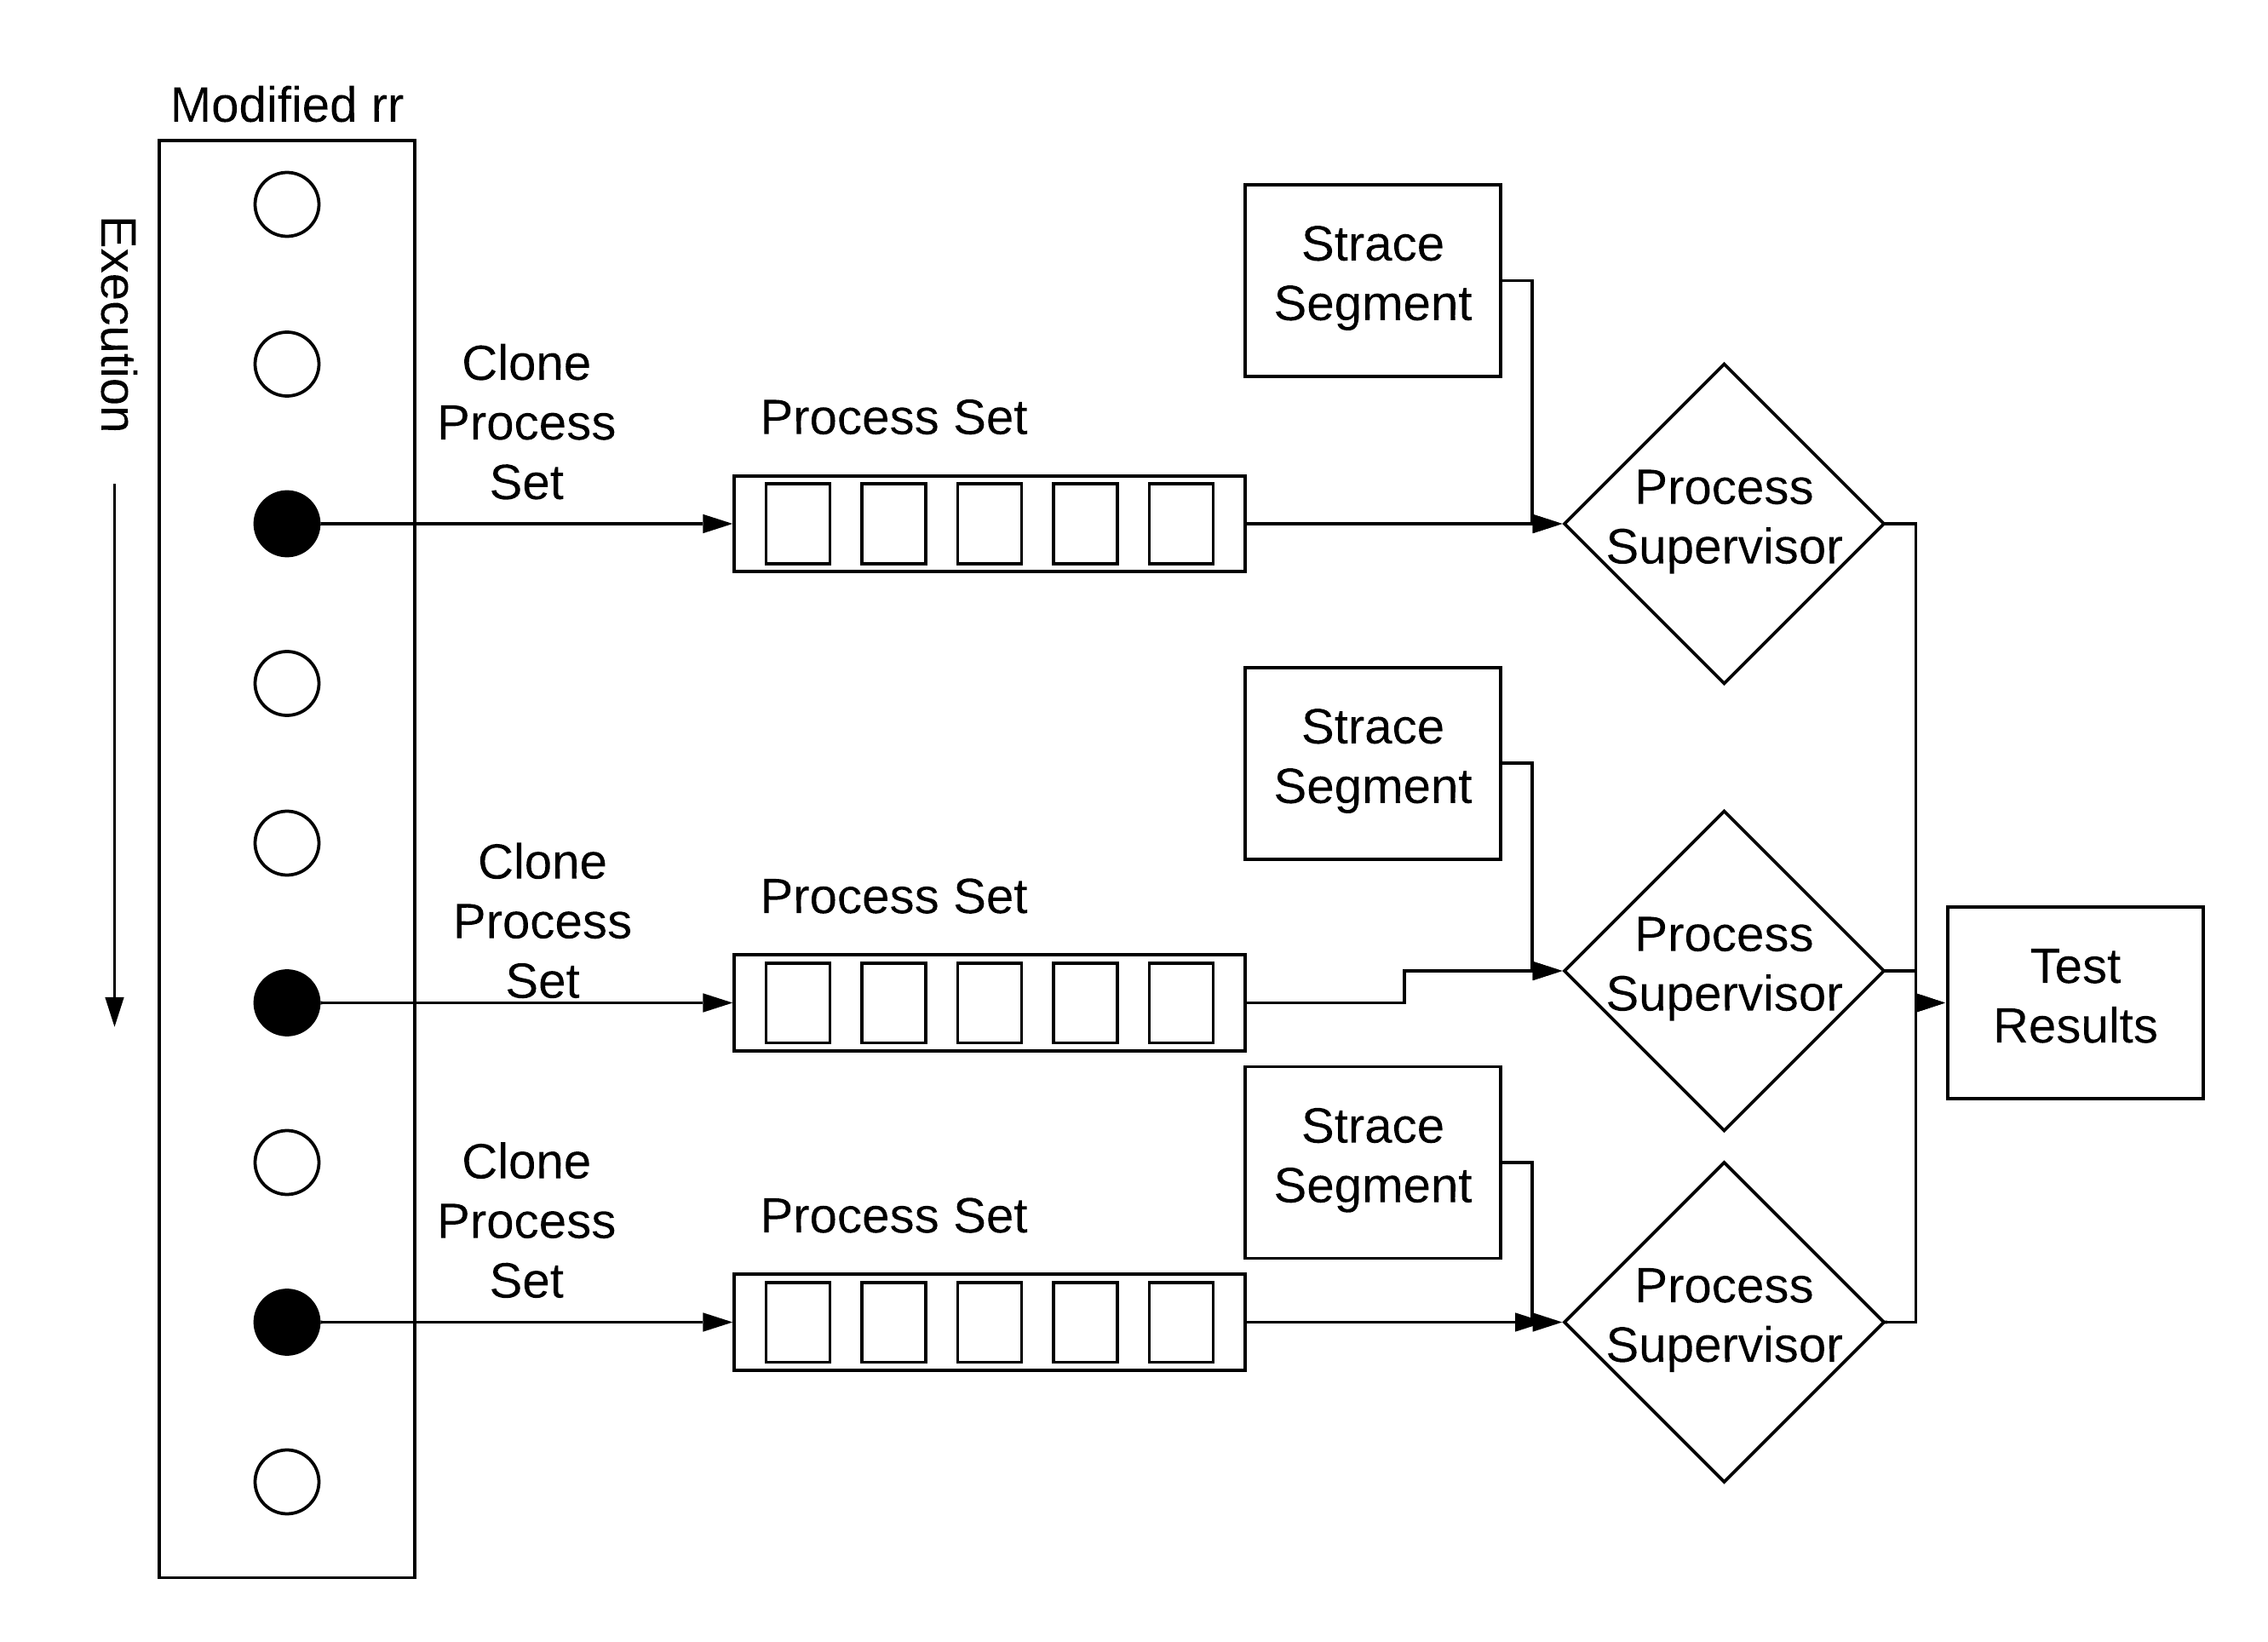
\includegraphics[scale=.65]{images/architecture}}
  \caption{Diagram illustrating CrashSimulator's Architecture.  During the
    course of a single rr execution, clone process sets are generated at
    specific rr events.  A CrashSimlator supervisor process attaches to
    these process sets and uses a strace-style system call listing to feed
    subsequent system call activity and inject unusual environmental
    conditions.}
  \label{figure:architecture}
\end{figure*}

As mentioned earlier,
the Simulating Environmental Anomalies(SEA)
offers a methodical way to identify bugs that could arise from interaction
with a given environment.
It does this by providing a systematic way of
capturing, storing and utilizing the insights gleaned from the work that
went into debugging previous failures in a given environment.
In this section, we offer a high-level look at how SEA works, followed by
a more in-depth look at its primary operations.
Finally, we detail our concrete implementation, CrashSimulator.

\subsection{SEA in a Half-shell}
\label{SEC:SEAHalfshell}
In a nutshell,
here is how the technique works.
An application is run
in a particular environment and fails.
In debugging the failure,
we identify and ``trap'' the particular environmental feature
(sec.~\ref{SUBSUB:IdentifyingAndEncoding}),
that caused the failure,  which we call $X$.
We verify that when $X$ is present,
communication with the
environment is different,
sometimes in a barely perceptible manner,
and other times in a radically contrary manner.
We call this difference $X'$.
$X'$ can be extracted, preserved,
and later used in testing other systems
thanks to a pair of components referred to as a mutator and a checker.
The mutator describes $X'$ as an exact set of changes
that must be made to an application's communications
in order to simulate $X$,
while the checker describes how an
application should respond once the $X$ has been encountered.
To test if other applications also have a problem with $X$,
mutators can insert $X'$ into their
communications (sec.~\ref{SUBSUB:MutatingCommunications}).
A checker will then determine whether the
application has responded correctly to
$X$(sec.~\ref{SUBSUB:CheckingResponse}).
If the checker accepts the application behavior
after the anomaly is simulated,
we report it has been handled.
If the checker doesn't accept we report that it hasn't.
Once created,
these pieces act as the persistent medium in which the details of
a given anomaly are stored.

Preserving this information in an accessible manner
is a boon for software developers because,
in a typical scenario, the material documenting
the discovery of flaws
either goes out of date or
is preserved only as ``institutional memory,''
and therefore forgotten as staffs change.
Additionally,
the mere existence of documentation
describing past failures
does not prevent bugs
if developers don't use it
to construct and execute tests,
an effort that is easily neglected.
Further, unit and integration test suites
are typically tightly coupled
to the application and the programming language in which it was written --
limiting their reusability.
SEA cuts through all of these difficulties by
storing this information in a manner that can be consumed
and used to test applications programmatically.
In this section, we discuss each of the components
required to implement SEA
and detail our concrete implementation,
CrashSimulator~\ref{SUBSEC:ApproachCrashSim}.

\subsection{Primary Operations}
\label{SEC:PrimaryOperations}

To take a closer look at how SEA functions,
we divide the technique
into its three primary operations.
These are:
identifying and trapping anomalies,
mutating system call results,
and checking application responses.

\subsubsection{Identifying and Encoding Anomalies}
\label{SUBSUB:IdentifyingAndEncoding}
At the core of SEA's operation is the body of anomalies
used to test applications.
Building this corpus is an ongoing process that improves the technique's
effectiveness by extending the set of anomalies it can simulate.
Anomalies can be sourced
in a number of ways,
such as
examining the failures of other applications
in a target deployment environment,
or by using other tools that can identify
potentially problematic behavior in other domains~\cite{Zhuang_NSDI_2014,
rasley2015detecting}.
Public bug trackers are an ideal source
if you wish to determine
whether or not an application
is vulnerable to a widely publicized bug.
The chosen anomalies are then examined
to determine how they change the results
of system calls an application makes
compared to a normal execution and why.
Once teased out,
these differences delineate
a set of modifications
that must be made
in order to simulate the chosen anomaly or anomalies.
These details are used to
construct both a mutator and a checker.
The mutator encodes
a description of when in execution an anomaly can be simulated
and the details of how to simulate it.
The checker
(or set of checkers)
stores a characterization of
how the application should respond.
Describing anomalies in this fashion
allows them to be recorded systematically and cataloged for future use.

Consider,
for example,
an anomalous environment
where access to a required file is denied because of
the environment's file security configuration.
With this anomaly,
attempts to access the file
such as calls to {\tt fread()},
or the {\tt read()} system call,
will fail with an error stating that access to the file is denied.
The mutator derived from this issue would be constructed to
identify similar accesses as opportunities
to simulate the anomaly
and carry out this simulation
by making these
accesses return ``access denied''.
As described in \ref{SUBSUB:CheckingResponse},
an associated checker would be built to
examine the application's behavior after a simulation and assess its
correctness.
Preserving the details of this anomaly
as a mutator and checker
allows them to be
easily used
to see how future applications
respond to this anomaly.

\subsubsection{Mutating System Call Results}
\label{SUBSUB:MutatingCommunications}
Simulating an environmental anomaly requires specific interventions at the
correct moments during an execution.
These situations are identified
with the help of the chosen anomaly's
mutator.
In practice,
this means providing the
mutator with the system calls
the application makes
so that it can identify sequences
indicative of such opportunities.
At the appropriate time,
the application's system calls
are intercepted
and the mutator's anomaly description is used to
make the modifications necessary
to simulate the anomaly.
In the simplest case,
simulating an anomaly only requires
the modification of a single value.
In more complex cases,
large numbers of diverse system calls
need to be interdicted and altered
in order to correctly simulate an anomaly.
The above file access scenario, for example,
requires the modification of a single system call.
Simulating something more complex,
like an unreliable system clock,
requires that all efforts
to access the clock
be modified to reflect the chosen aberration.

\subsubsection{Checking an Application's Response}
\label{SUBSUB:CheckingResponse}
SEA relies on checkers
to provide a flexible approach to assess the way an application
behaves after it has encountered an anomaly.
A checker is constructed to store
some behavior that the application should undertake
in response to simulated anomaly.
It looks for this behavior by examining an application's system calls
before, during, and after the simulation of an anomaly.
The checker then reports whether the application has handled
the anomaly based on whether or not it observed the behavior for which it
was built to look.

As an example, consider the ``default checker'' from CrashSimulator.
It draws a conclusion based on
whether or not the application
has made an effort to respond
to the anomaly.
This determination is made based
on the assumption
that such a response will yield
different program paths (and therefore different system calls).
If the application
does not alter its behavior, it has not
correctly handled this flaw.
Alternatively,
if the application does deviate,
it is likely
an action has occurred to handle the simulated condition.
This simple yes or no approach
is often sufficient
to classify application behavior.



\subsection{CrashSimulator: A Concrete SEA Implementation}
\label{SUBSEC:ApproachCrashSim}
The construction of CrashSimulator,
our concrete implementation of SEA,
was driven by two key decisions.
The first
was to operate at the system call level,
rather than manipulating
calls to library functions, memory accesses, or other points where we could
influence an application's communications.
System calls are high enough level that they allow us
to ignore low level details that would hurt usability while still
capturing the environmental anomalies we are interested in.
They also provide us with a
few technical advantages.
First, there is already robust tooling in the Linux
kernel that allows for the interception and modification of system call
results and side effects.  Additionally, Linux system call semantics are
well defined which simplifies implementation. Finally, operating at this
level allows CrashSimulator to test applications written in any language
that can execute Linux system calls.

The second decision was to structure testing around recording and replaying
applications.  This was done to make tests trivially repeatable and to ease
the process of manipulating system calls.  Recording and replay was
achieved using the {\tt rr} debugger~\cite{rrwebsite}.
Some modifications to {\tt rr} were required in order to
tailor it more closely to our needs.
These modifications allow
a {\tt strace}-style
system call recording to be output alongside {\tt rr's} normal recording
format, providing
a complete log of an application's system call activity.
We chose to make this
modification because {\tt rr} is concerned with execution
at the level of individual instructions and memory accesses while the
anomalies we were interested in were more in terms of
system calls.

These anomalies (which are discussed
in Section~\ref{SEC:evaluation})
were collected by examining public bug trackers,
the source code of major portable applications, and the capabilities of
tools like NetCheck~\cite{Zhuang_NSDI_2014}
and CheckAPI~\cite{rasley2015detecting}.
From these anomalies,
we constructed
checkers and mutators
using finite automata.
Mutators work by receiving the sequence of system calls
an application makes and accepting situations where the sequence indicates
it is appropriate to simulate an anomaly.
It then uses its stored
description of an anomaly
to carry out its simulation.
Checkers operate similarly,
but, because they encode what a
correct response by the application should look like,
they were constructed
to accept situations where they observed sequences indicative of such
behavior.

Actually simulating anomalies
is done using
a technique
we call {\it process set cloning}.
The {\tt rr} debugger manages,
and can copy,
the full set of processes underlying an application
so that users can test debugging
hypotheses without damaging the original.
We extended this capability
by liberating process set copies from {\tt rr}.
This means that given application $Y$
consisting of processes $a$, $b$, and $c$
(written as $Y(a, b, c)$),
we can generate cloned sets $Y_1(a_1, b_1, c_1)$,
$Y_2(a_2, b_2, c_2)$ ... $Y_n(a_n, b_b, c_n)$.
$Y_1$, $Y_2$ ... $Y_n$ can then be used to test different scenarios leaving
the original $Y$ to continue its execution unhindered.
Process sets generated in this fashion are created in a stopped state and
remain that way until they are attached to and utilized by a CrashSimulator
supervisor.

Once a supervisor has attached to a process set, it uses the above {\tt
strace} log and the output of a mutator to service any future
system calls the application makes.  In this way, the mutator is able to
influence system call results and simulate its anomaly.
During this process,
a corresponding checker
monitors the application's behavior,
allowing it to report on the correctness of the response.
For example, testing could proceed in the following way.
At a given point in the execution of application $Y$,
cloned sets $Y_1$ and $Y_2$ are generated and
used to test two scenarios where a file access could fail:
\begin{enumerate}
    \item{For $Y_1$, access to the file is denied due to a permissions issue}
    \item{For $Y_2$, access fails because of an I/O error}
\end{enumerate}
The simulations for both $Y_1$ and $Y_2$ are handled asynchronously and
the results reported.
This approach allows many tests to be run independently of one another,
which lends a
high degree of speed and
parallelism to the testing process.
At the same time, the original $Y$ execution continues unhindered to the
next simulation opportunity where this process repeats.
Keeping $Y$ intact
(as opposed to destroying it by introducing an error state)
avoids the penalty
of having to restart a new execution for each test.

The prototype was built on rr version 5.2.0 running on a 32-bit Linux kernel
distributed with Ubuntu 16.04 LTS.  The modifications to rr, which are
explained in this section, were carried out in C++ and the CrashSimulator
supervisor was implemented in ZZZZ lines of Python 2.7 code with a YYYY
line C extension that allows it to interact with processes using the Ptrace
API.
This version of CrashSimulator is available as a Docker container and,
due to some operating system configuration being necessary, is most easily
installed in this fashion.
